\section{Current status of searches for charged Higgs}
\label{s:searchHplus}
There have been several searches for the charged Higgs boson in last two decades, 
particularly in the context of Type II of the 2HDM. However, no signature of the 
existence of the charged Higgs has been found
as of now. In the absence of any signal for the charged Higgs, various constraints
have been imposed from a wide range of theoretical studies as well as low and high energy 
collider experiments. The theoretical constraints come from the vacuum stability,
perturbative unitarity, and electro-weak precision observables 
\cite{Arhrib:2018ewj}. The low energy constraints are from the indirect searches
\cite{Akeroyd:2016ymd} where a charged Higgs appears in the loop such as the 
decay of B-mesons ($B \rightarrow X_s\gamma$). The high energy constraints are 
from the direct production of charged Higgs at the collider experiments 
\cite{Achard:2003gt, Heister:2002ev, Abdallah:2003wd, Abbiendi:2008aa,
Aaltonen:2009ke,Abazov:2009aa,Aad:2013hla,Khachatryan:2015uua}. The constraints 
from direct searches are more reliable as compared to those from indirect searches 
or theoretical predictions.

The direct searches of the charged Higgs have been performed at the different
experiments such as ALEPH, L3, DELPHI, and OPAL at the large electron-positron 
collider (LEP), D0 and CDF at the Tevatron, and finally CMS and ATLAS at the large hadron
collider (LHC) in different decay channels of the charged Higgs. These searches
have been performed at different center of mass energies, different luminosities,
and for a wide range of the mass of the charged Higgs boson. Constraints have
been imposed on various parameters such as the mass of charged Higgs, $\tan\beta$, 
branching ratio of \PQt quark decay into the charged Higgs and \PQb quark, etc. A 
summary of all constraints from the collider experiment is shown in Tables 
\ref{tab:searchHplus1} and \ref{tab:searchHplus2}. The current best constraints 
are: \mHp $\textgreater$ 79.3 \GeV from the ALEPH at 0.2 \TeV (0.63\fbinv), 
\brThb $\textless$ 0.8-0.5\% for \mHp in range 90 to 150 \GeV at 13 \TeV 
(35.9\fbinv) from the CMS experiment, \sigHp $\times$ \brHtv $\textless$ 
4.2-0.0025\unit{pb} for \mHp in range 90 to 2000 \GeV at 13 \TeV (36.1\fbinv) from 
the ATLAS, \sigHp $\times \mathcal{B}(\text{H}^+ \rightarrow \text{t}\bar{\text{b}})$  $\textless$ 
9.6-0.01\unit{pb} for \mHp in range 200 to 3000 \GeV at 13 \TeV (35.9\fbinv) from 
the CMS, and all $\tan\beta \textgreater $ 1 values are excluded for \mHp up to 
160 \GeV from both CMS as well as ATLAS. A few of the current best constraints 
are shown in Figure~\ref{fig:searchHplus}.
\begin{table}
	\caption{Allowed range at 95\% CL for various parameters from the search 
	for charged Higgs involving $c\bar{s}$ channel at different collider 
	experiments.}
	\label{tab:searchHplus1}
\begin{centering}
\begin{tabular}{ccp{3cm}p{5cm}p{3cm}}
	\hline
	\hline
	Experiment & Year & $\sqrt{s}$ ($\lumi_{int}$) & Allowed range at 95\% CL
	& Assumption \\ \noalign{\vskip 0.2cm} 
	& 	& \TeV (\fbinv)    &  	&\\
	\hline
	\hline \noalign{\vskip 0.2cm}
	ALEPH 	& 2002 \cite{Heister:2002ev} & 0.189-0.209 (0.629) & \mHp 
	$\textgreater$ 79.3 \GeV  & 
	\brHtv + \brHcs = 1\\ \noalign{\vskip 0.2cm}
	L3 	& 2003 \cite{Achard:2003gt} & 0.189-0.209 (0.629) & \mHp 
	$\textgreater$ 76.5 \GeV  & 
	\brHtv + \brHcs = 1\\ \noalign{\vskip 0.2cm}
	DELPHI 	& 2004 \cite{Abdallah:2003wd} & 0.189-0.209 (0.220) & \mHp 
	$\textgreater$ 74.5 \GeV  & 
	Pair production of $ H^+H^-$ in channels 
	$\tau^+\nu_\tau\tau^-\bar{\nu}_\tau, ~c\bar{s}\bar{c}s, 
	~c\bar{s}\tau^-\bar{\nu}_\tau$
	\\ \noalign{\vskip 0.2cm}
	OPAL 	& 2012 \cite{Abbiendi:2008aa} & 0.189-0.209 (0.6) & \mHp 
	$\textgreater$ 76.3 \GeV & 
	\brHtv + {\ensuremath{\mathcal{B}(H^+ \rightarrow \text{q}\text{q}^\prime)}\xspace} = 1
	\\ \noalign{\vskip 0.2cm}
	\hline
	CDF 	& 2009 \cite{Aaltonen:2009ke}& 1.96 (2.2) & \brThb $\textless$ 
	10-30\%, for \mHp in 
	range 60 to 150 \GeV& \brHcs = 1\\ \noalign{\vskip 0.2cm}
	D0 	& 2009 \cite{Abazov:2009aa} & 1.96 (1.0) & \brThb $\textless$ 
	22\%, for \mHp in 
	range 80 to 155 \GeV& \brHcs = 1\\ \noalign{\vskip 0.2cm}
	\hline
	ATLAS 	& 2013 \cite{Aad:2013hla} & 7 (4.7) & \brThb $\textless$ 5.1\%, 
	for \mHp in 
	range 90 to 150 \GeV& \brHcs = 1\\ \noalign{\vskip 0.2cm}
	CMS 	& 2016 \cite{Khachatryan:2015uua} & 8 (19.7) & \brThb $\textless$ 
	6.5-1.2\%, for \mHp in 
	range 90 to 150 \GeV& \brHcs = 1\\ \noalign{\vskip 0.2cm}
	CMS 	& 2019 & 13 (35.9) & \textcolor{red}{Presented in 
	this thesis} & \brHcs = 1\\ \noalign{\vskip 0.2cm}
	\hline
	\end{tabular}
	\par\end{centering}
\end{table}


\begin{table}
	\caption{Allowed range at 95\% CL for various parameters from the search 
	for charged Higgs involving other channels such as $\tau^+\nu, ~c\bar{b}$, 
	and $t\bar{b}$ at different collider experiments.}
	\label{tab:searchHplus2}
\begin{centering}
%\begin{tabular}{cccccc}
\begin{tabular}{ccp{2.0cm}p{6cm}p{3.5cm}}
	\hline
	\hline
	Experiment & Year & $\sqrt{s}$ ($\lumi_{int}$) & Allowed range at 95\% CL
	& Assumption \\ \noalign{\vskip 0.2cm} 
	& 	& \TeV (\fbinv)    &  	&\\
	\hline
	\hline \noalign{\vskip 0.2cm}
	D0 	& 2009 \cite{Abazov:2009aa} & 1.96 (1.0) & \brThb $\textless$ 
	15-19\%, for \mHp in range 80 to 155 \GeV& \brHtv = 1\\ \noalign{\vskip 0.2cm}
	ATLAS 	& 2013 \cite{Aad:2012rjx} & 7 (4.6) & \brThb $\textless$ 0.8-3.4\%, 
	for \mHp in range 90 to 160 \GeV& \brHtv = 1\\ \noalign{\vskip 0.2cm}
	ATLAS 	& 2015 \cite{Aad:2014kga} & 8 (19.5) & \sigHp$\times$\brHtv 
	$\textless$ 4.5-0.76\unit{pb} for \mHp in range 180 to 1000 \GeV, \brThb $\times$ 
	\brHtv $\textless$ 
	0.23-1.3\% for \mHp in range 80 to 160 \GeV, and $\tan\beta$ $\textless$ 
	1 for \mHp in range 80 to 160 \GeV& \brHtv = 1\\ \noalign{\vskip 0.2cm}
	ATLAS 	& 2016 \cite{Aaboud:2016dig} & 13 (3.2) & \sigHp $\times$ \brHtv 
	$\textless$ 1.9-0.015\unit{pb} for \mHp in range 200 to 2000 \GeV& \brHtv = 1\\ \noalign{\vskip 0.2cm}
	ATLAS 	& 2016 \cite{ATLAS:2016grc} & 13 (14.2) & \sigHp $\times$ \brHtv 
	$\textless$ 2.0-0.008\unit{pb} for \mHp in range 200 to 2000 \GeV& \brHtv = 1
	\\ \noalign{\vskip 0.2cm}
	ATLAS 	& 2018 \cite{Aaboud:2018gjj}& 13 (36.1) & \sigHp $\times$ \brHtv 
	$\textless$ 
	4.2-0.0025\unit{pb} for \mHp in range 90 to 2000 \GeV, \brThb $\times$ \brHtv 
	$\textless$ 0.25-0.031\% for \mHp in range 90 to 160 \GeV, and $\tan\beta$ 
	$\textless$ 1 is excluded for all \mHp up to 160 \GeV& \brHtv = 1
	\\ \noalign{\vskip 0.2cm}
	CMS 	& 2018 \cite{Sirunyan:2018dvm}& 8 (19.7) & \brThb $\textless$ 
	0.8-0.5\%, for \mHp in 
	range 90 to 150 \GeV& $\mathcal{B}(H^+\rightarrow \text{c}\bar{\text{b}})$ = 1\\ 
	\noalign{\vskip 0.2cm}
	CMS 	& 2019 \cite{Sirunyan:2019hkq}& 13 (35.9) & \sigHp $\times$ 
	\brHtv $\textless$ 
	6.0-0.005\unit{pb} for \mHp in range 80 to 3000 \GeV, and $\tan\beta$ $\textless$ 
	1 is excluded for all \mHp up to 160 \GeV& \brHtv = 1
	\\ \noalign{\vskip 0.2cm}
	CMS 	& 2019 \cite{CMS:1900zym} & 13 (35.9) & \sigHp $\times \mathcal{B} 
	(H^+\rightarrow t \bar{b})$ $\textless$ 9.6-0.01\unit{pb}, for \mHp in range 
	200 to 3000 \GeV & $\mathcal{B} (\text{H}^+\rightarrow \text{t} \bar{\text{b}})$ = 1
	\\ \noalign{\vskip 0.2cm}
	\hline
	\end{tabular}
	\par\end{centering}
\end{table}

\begin{figure}
\centering
\subfigure[Limit on \brThb \cite{Aad:2013hla}]{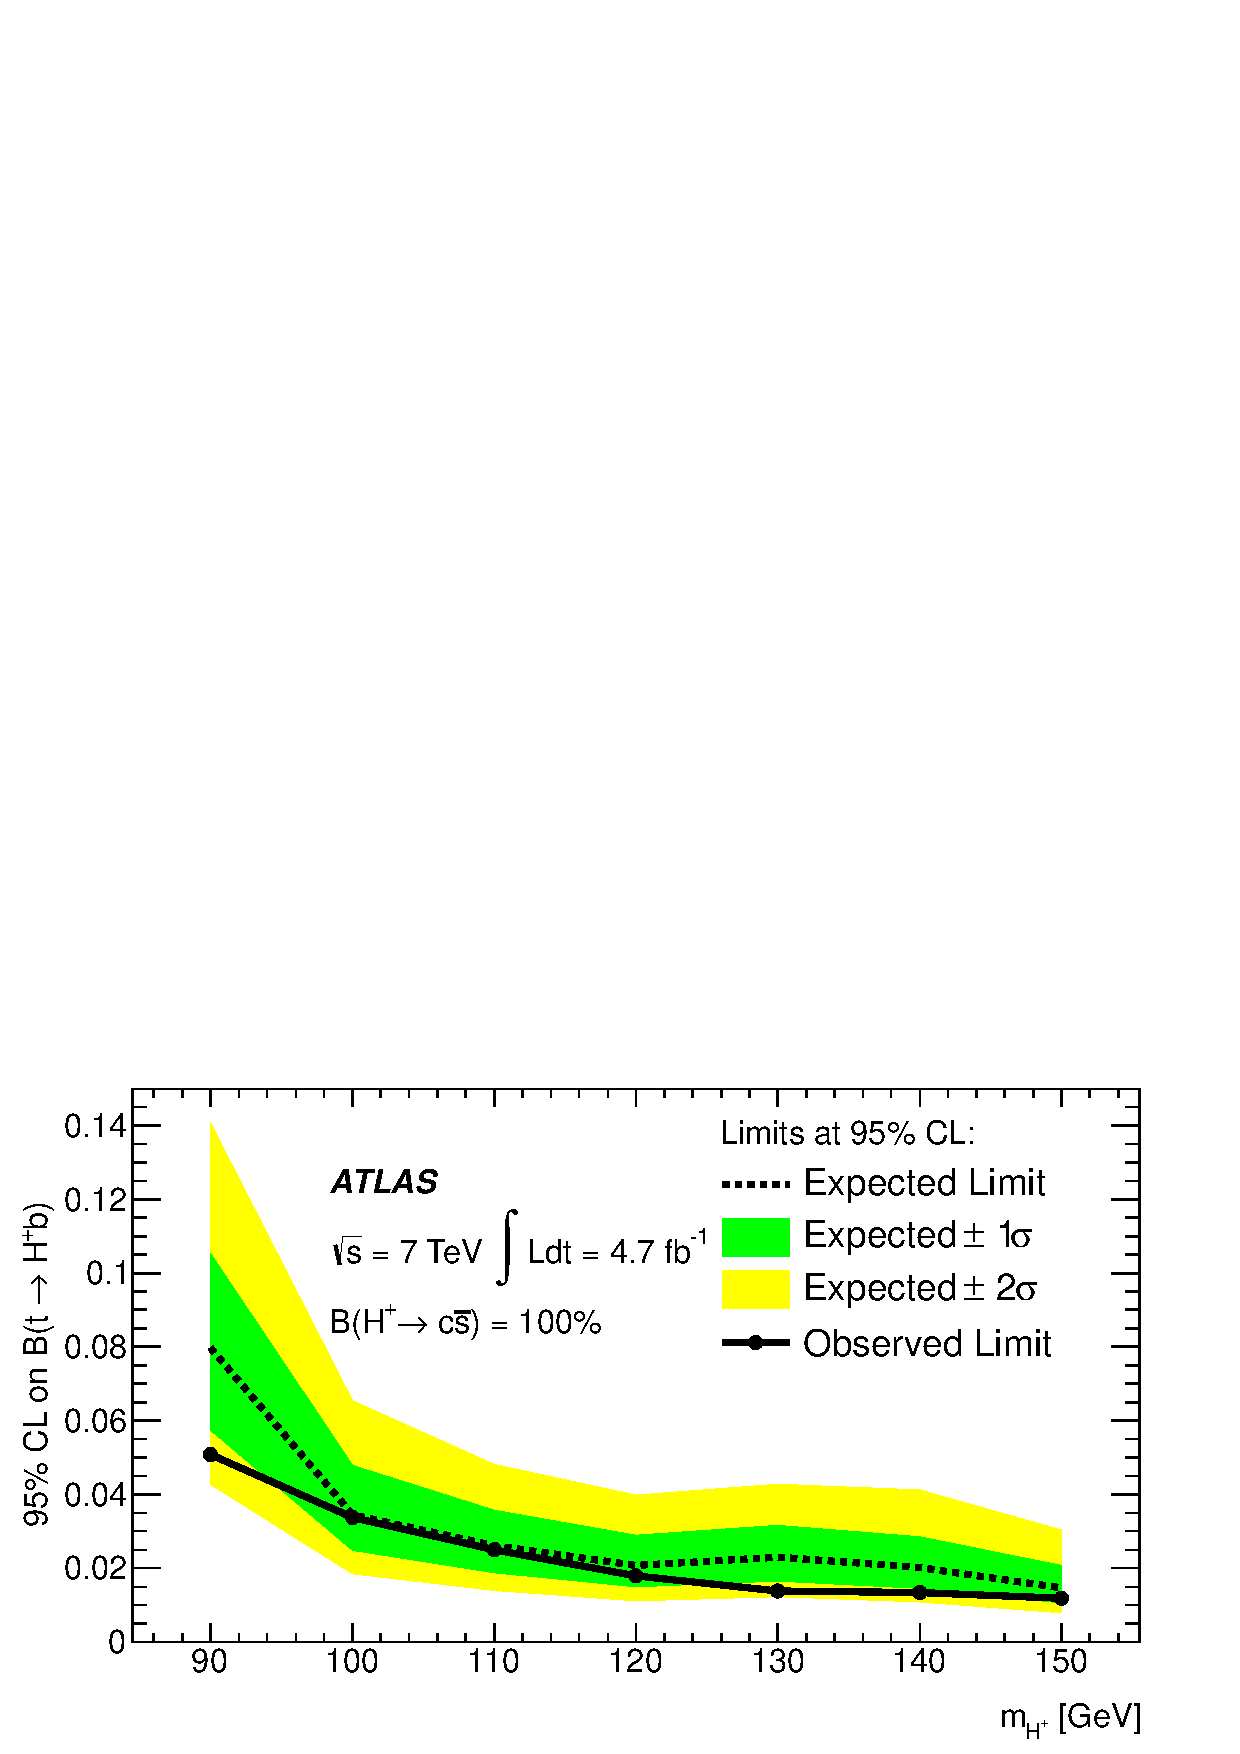
\includegraphics[width=0.50\linewidth]{Theory/Image/OldLimit/limit_atlas_csbar_7TeV.pdf}}
\subfigure[Limit on \sigHp$\times$\brHtv \cite{Aaboud:2018gjj}]{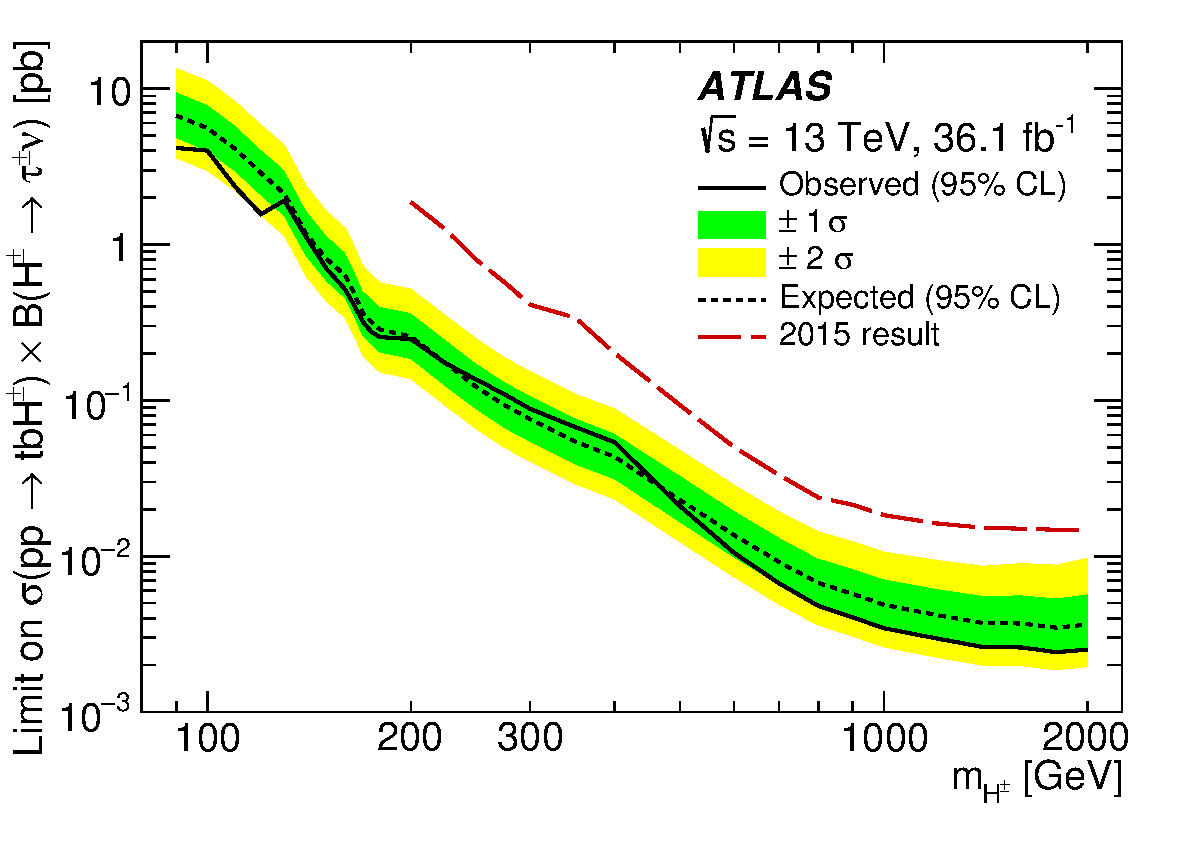
\includegraphics[width=0.40\linewidth]{Theory/Image/OldLimit/sigmaBR_atlas_13TeV_taunu.pdf}}
\vfil
\subfigure[Limit on \brThb \cite{Khachatryan:2015uua}]{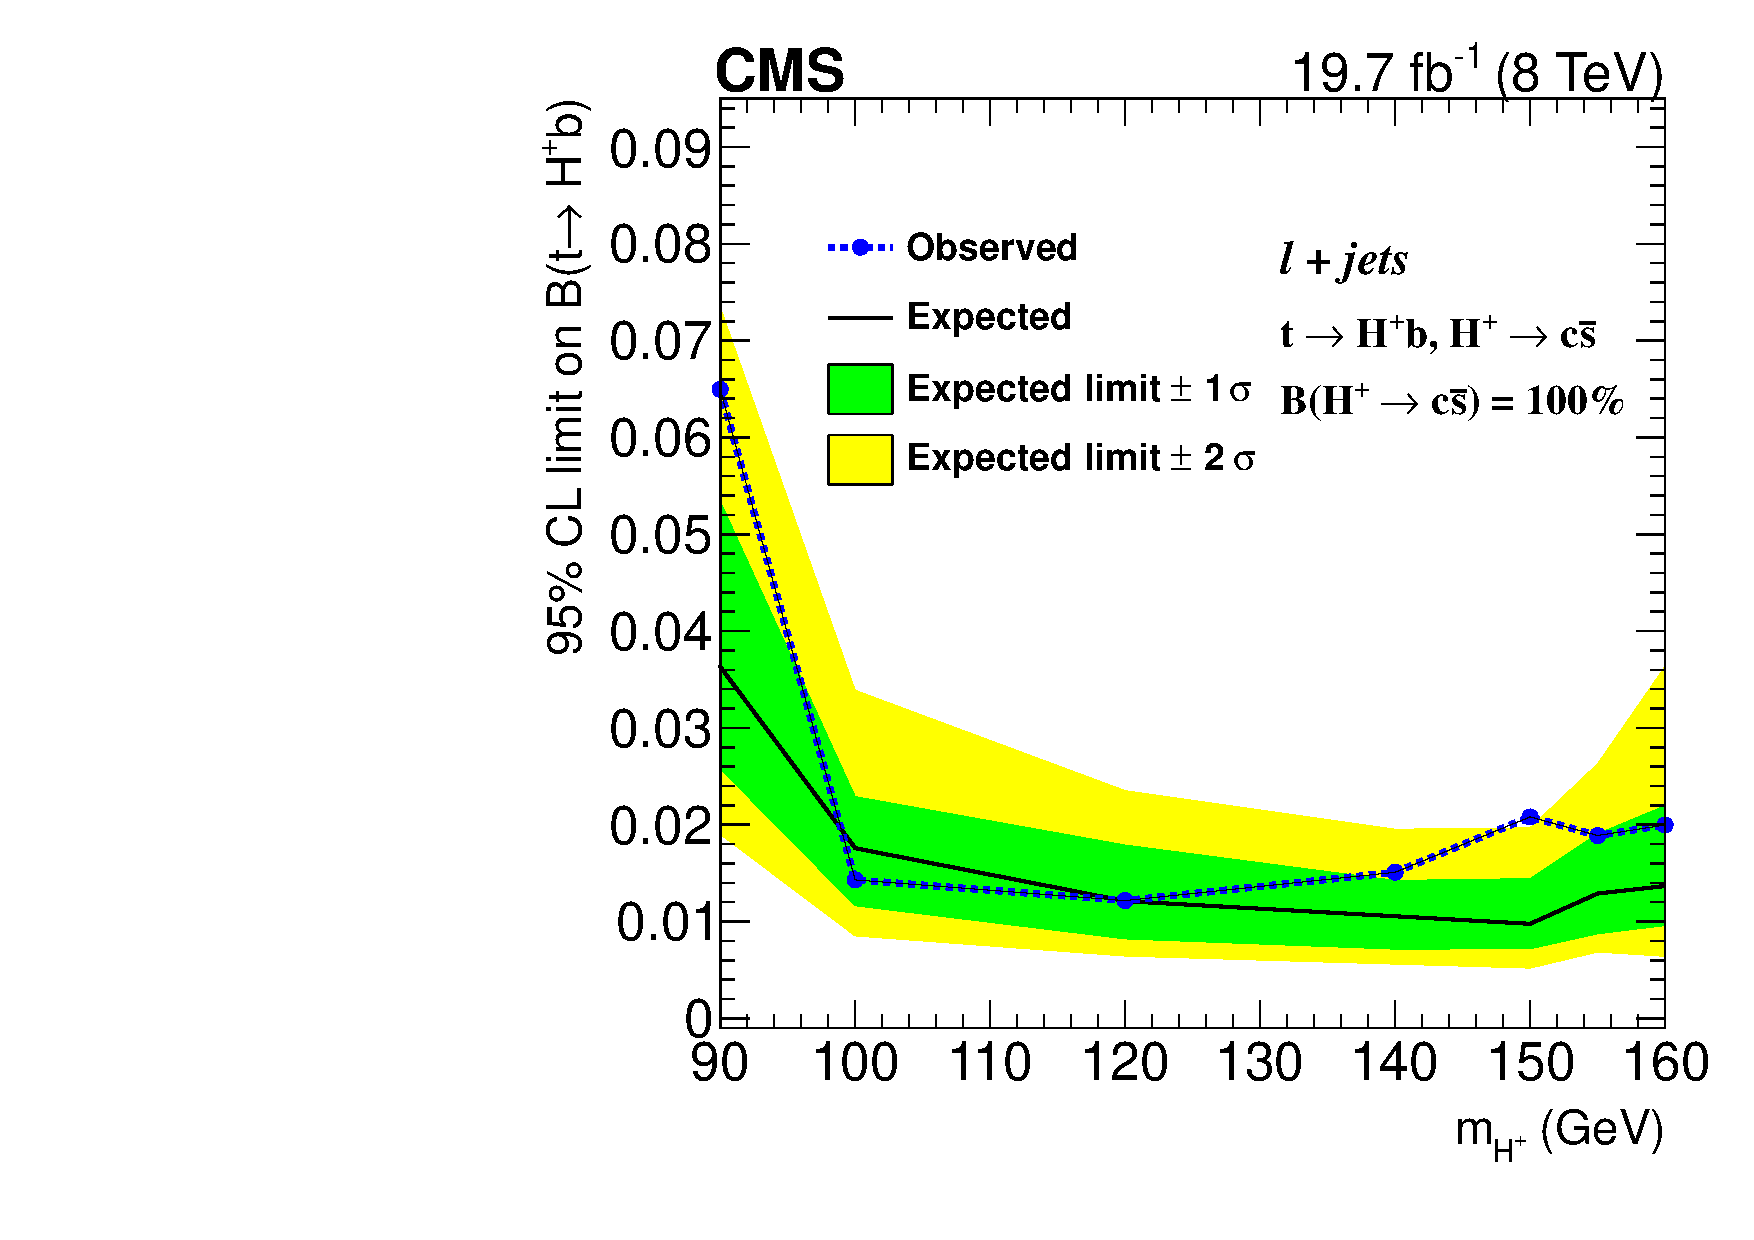
\includegraphics[width=0.45\linewidth]{Theory/Image/OldLimit/limit_CMS_csbar_8TeV.pdf}}
\subfigure[Limit on \sigHp$\times$\brHtv \cite{Sirunyan:2019hkq}]{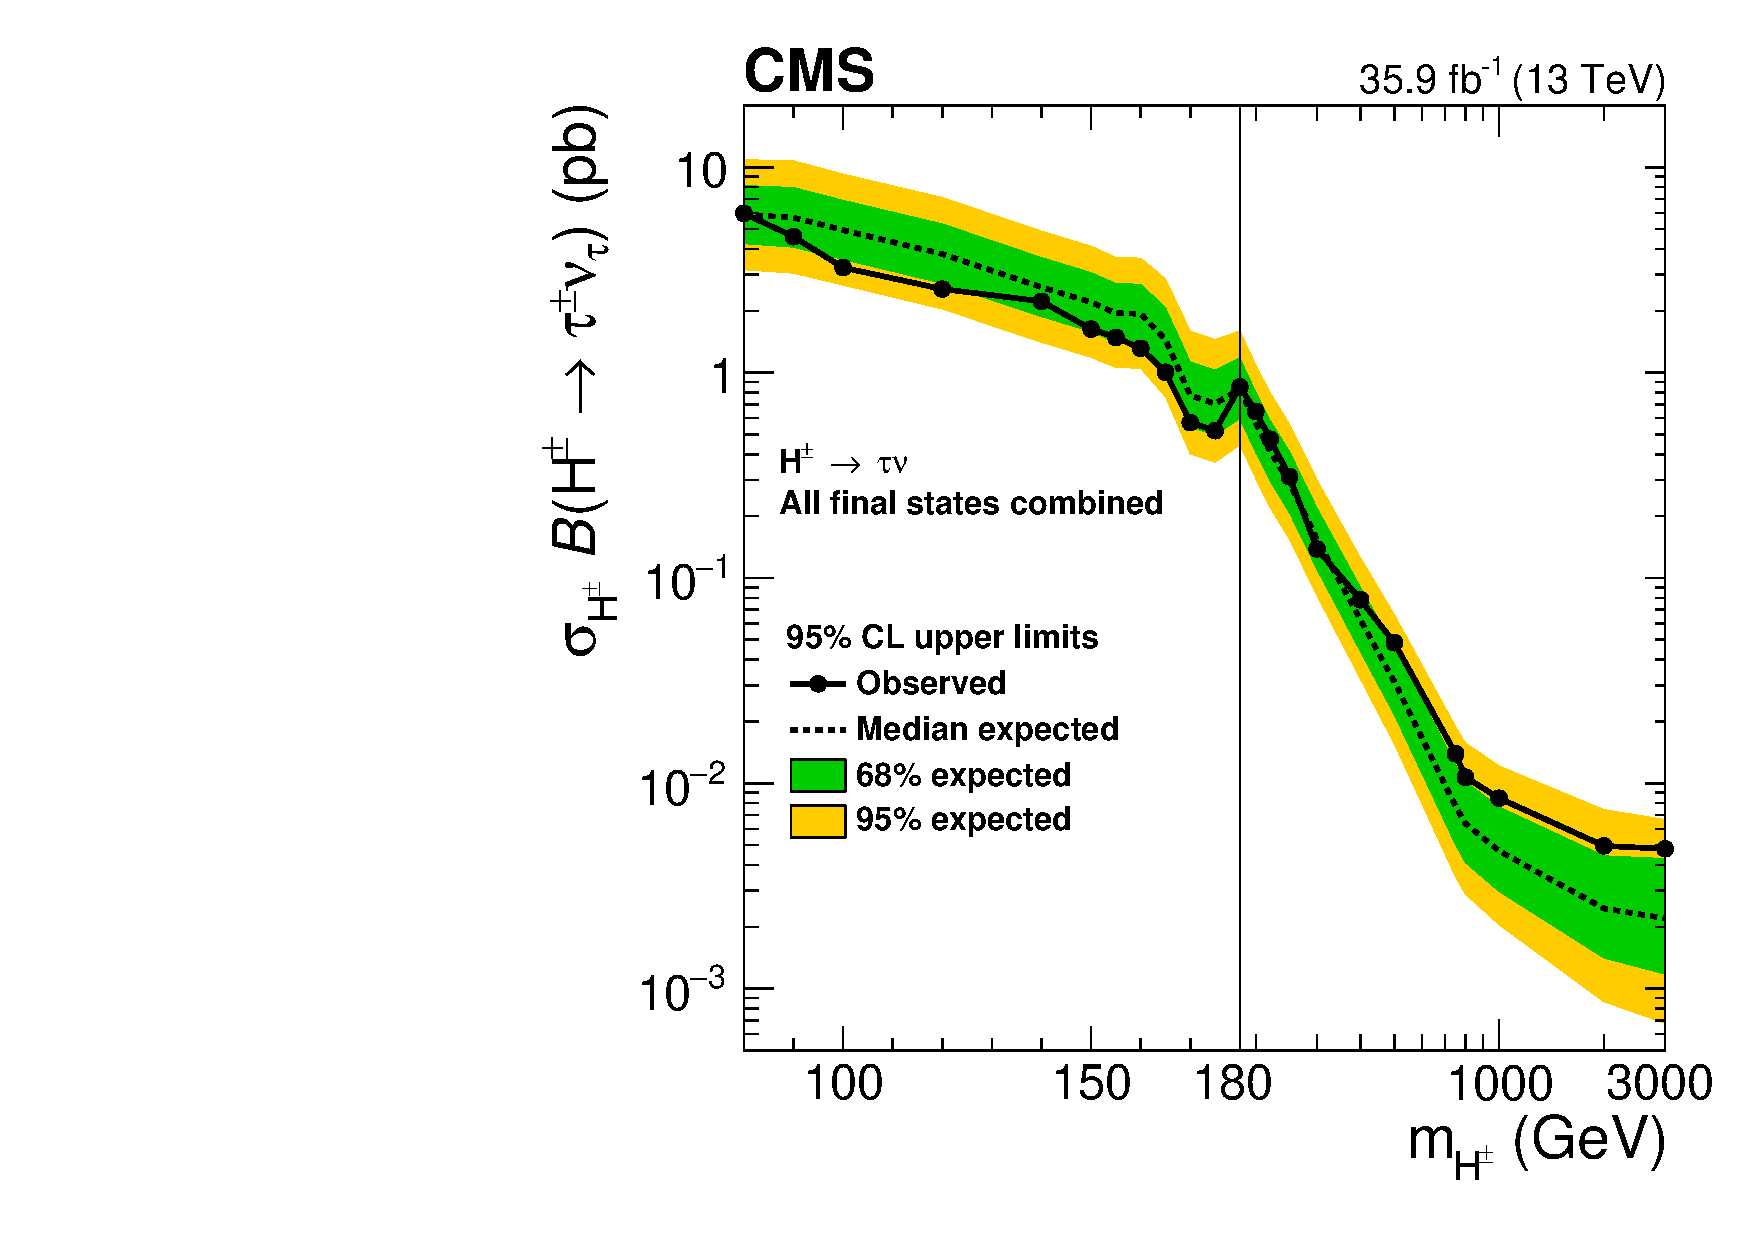
\includegraphics[width=0.45\linewidth]{Theory/Image/OldLimit/sigmaBR_cms_13TeV_taunu.pdf}}
\vfil
\subfigure[Limit in ($\tan\beta, ~\mHp$) plane \cite{Aaboud:2018gjj}]{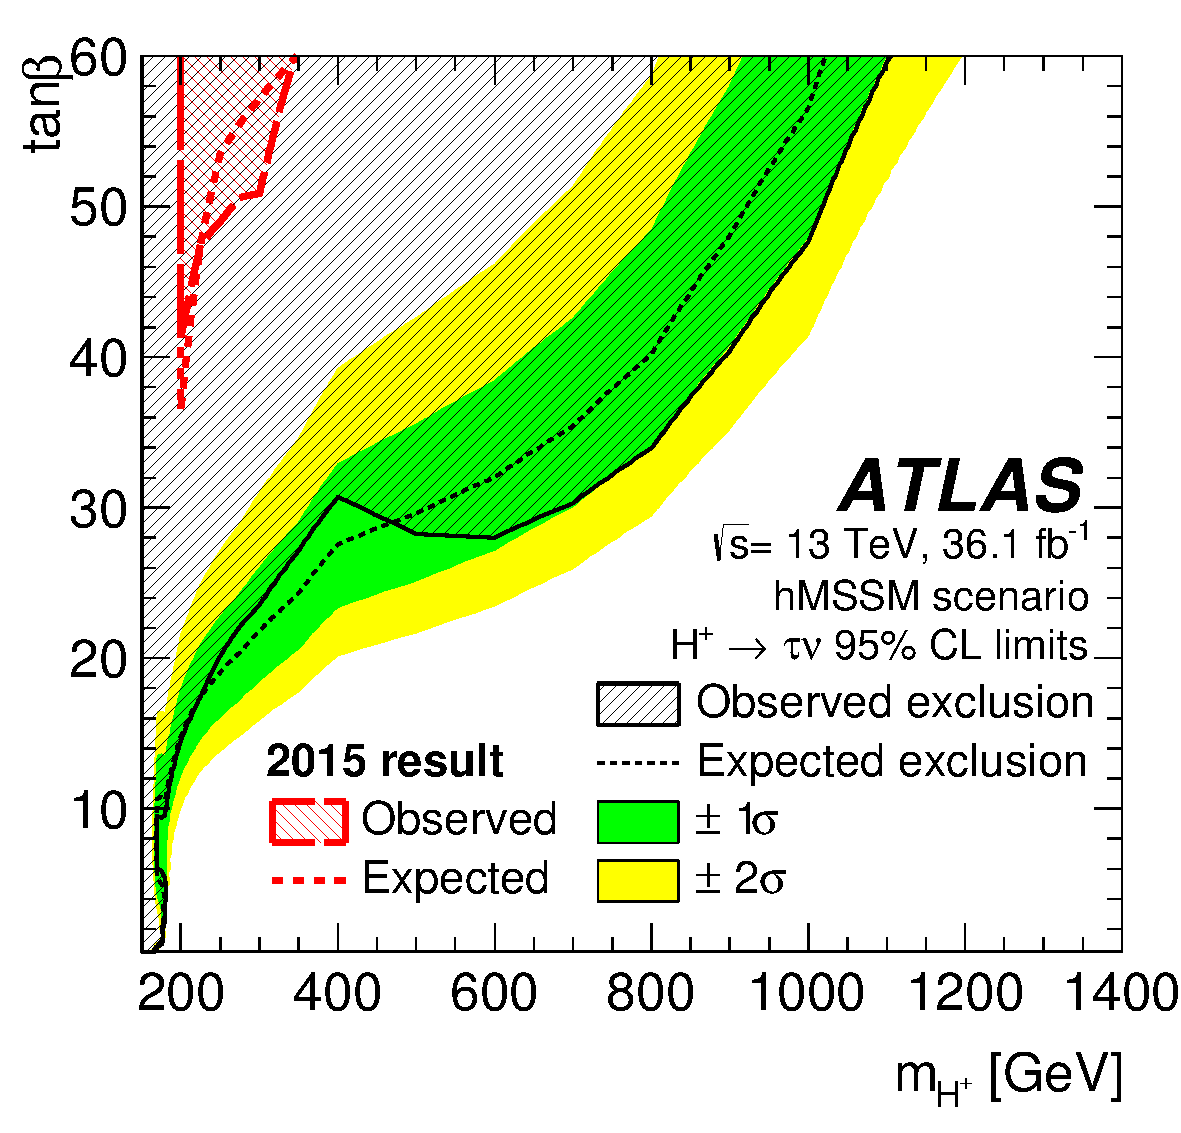
\includegraphics[width=0.45\linewidth]{Theory/Image/OldLimit/tanbeta_atlas_13TeV_taunu.pdf}}
\subfigure[Limit in ($\tan\beta, ~\mHp$) plane \cite{Sirunyan:2019hkq}]{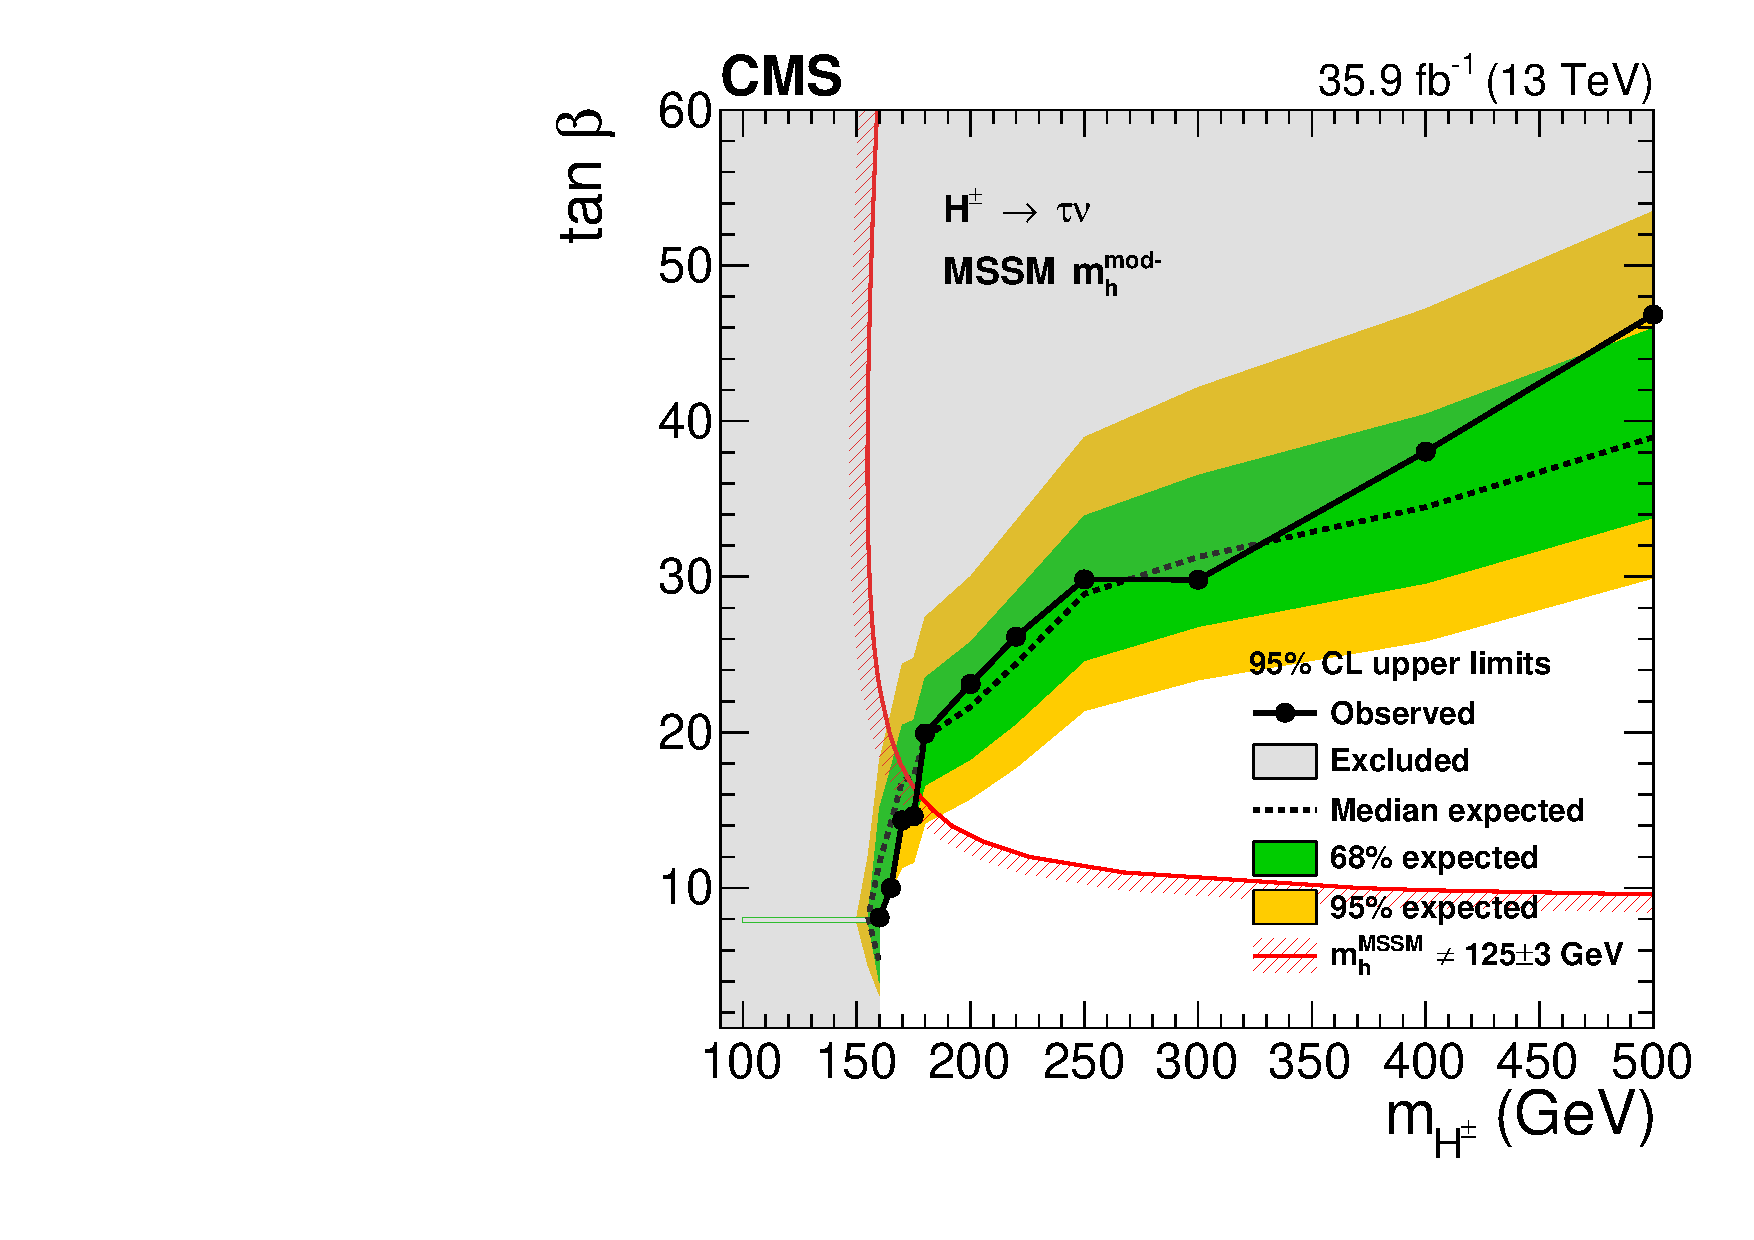
\includegraphics[width=0.45\linewidth]{Theory/Image/OldLimit/tanbeta_cms_13TeV_taunu.pdf}}
\caption{Current allowed range at 95\% CL from ATLAS and CMS.}
\label{fig:searchHplus}
\end{figure}



